\begin{figure}[htbp]
\centering
\captionsetup{
  justification=raggedright,
  labelsep=none,
  singlelinecheck=false,
  labelformat=boldlabel,
}
\caption[Hierarchical feature-importance decomposition.]{\footnotesize \textbf{: Hierarchical feature-importance decomposition.} Decomposition of feature importance from the individual signals through the base learners (OLS, GLMNET, RF, XGB, NN1--NN3) to the meta learner (the ML Ensemble). Nodes are signals, base learners and the meta learner; edge width and colour encode the importance each signal contributes to a base learner, and each base learner to the meta learner. Only the 10 most important signals per learner are shown. Estimated on the individual-signals run.}
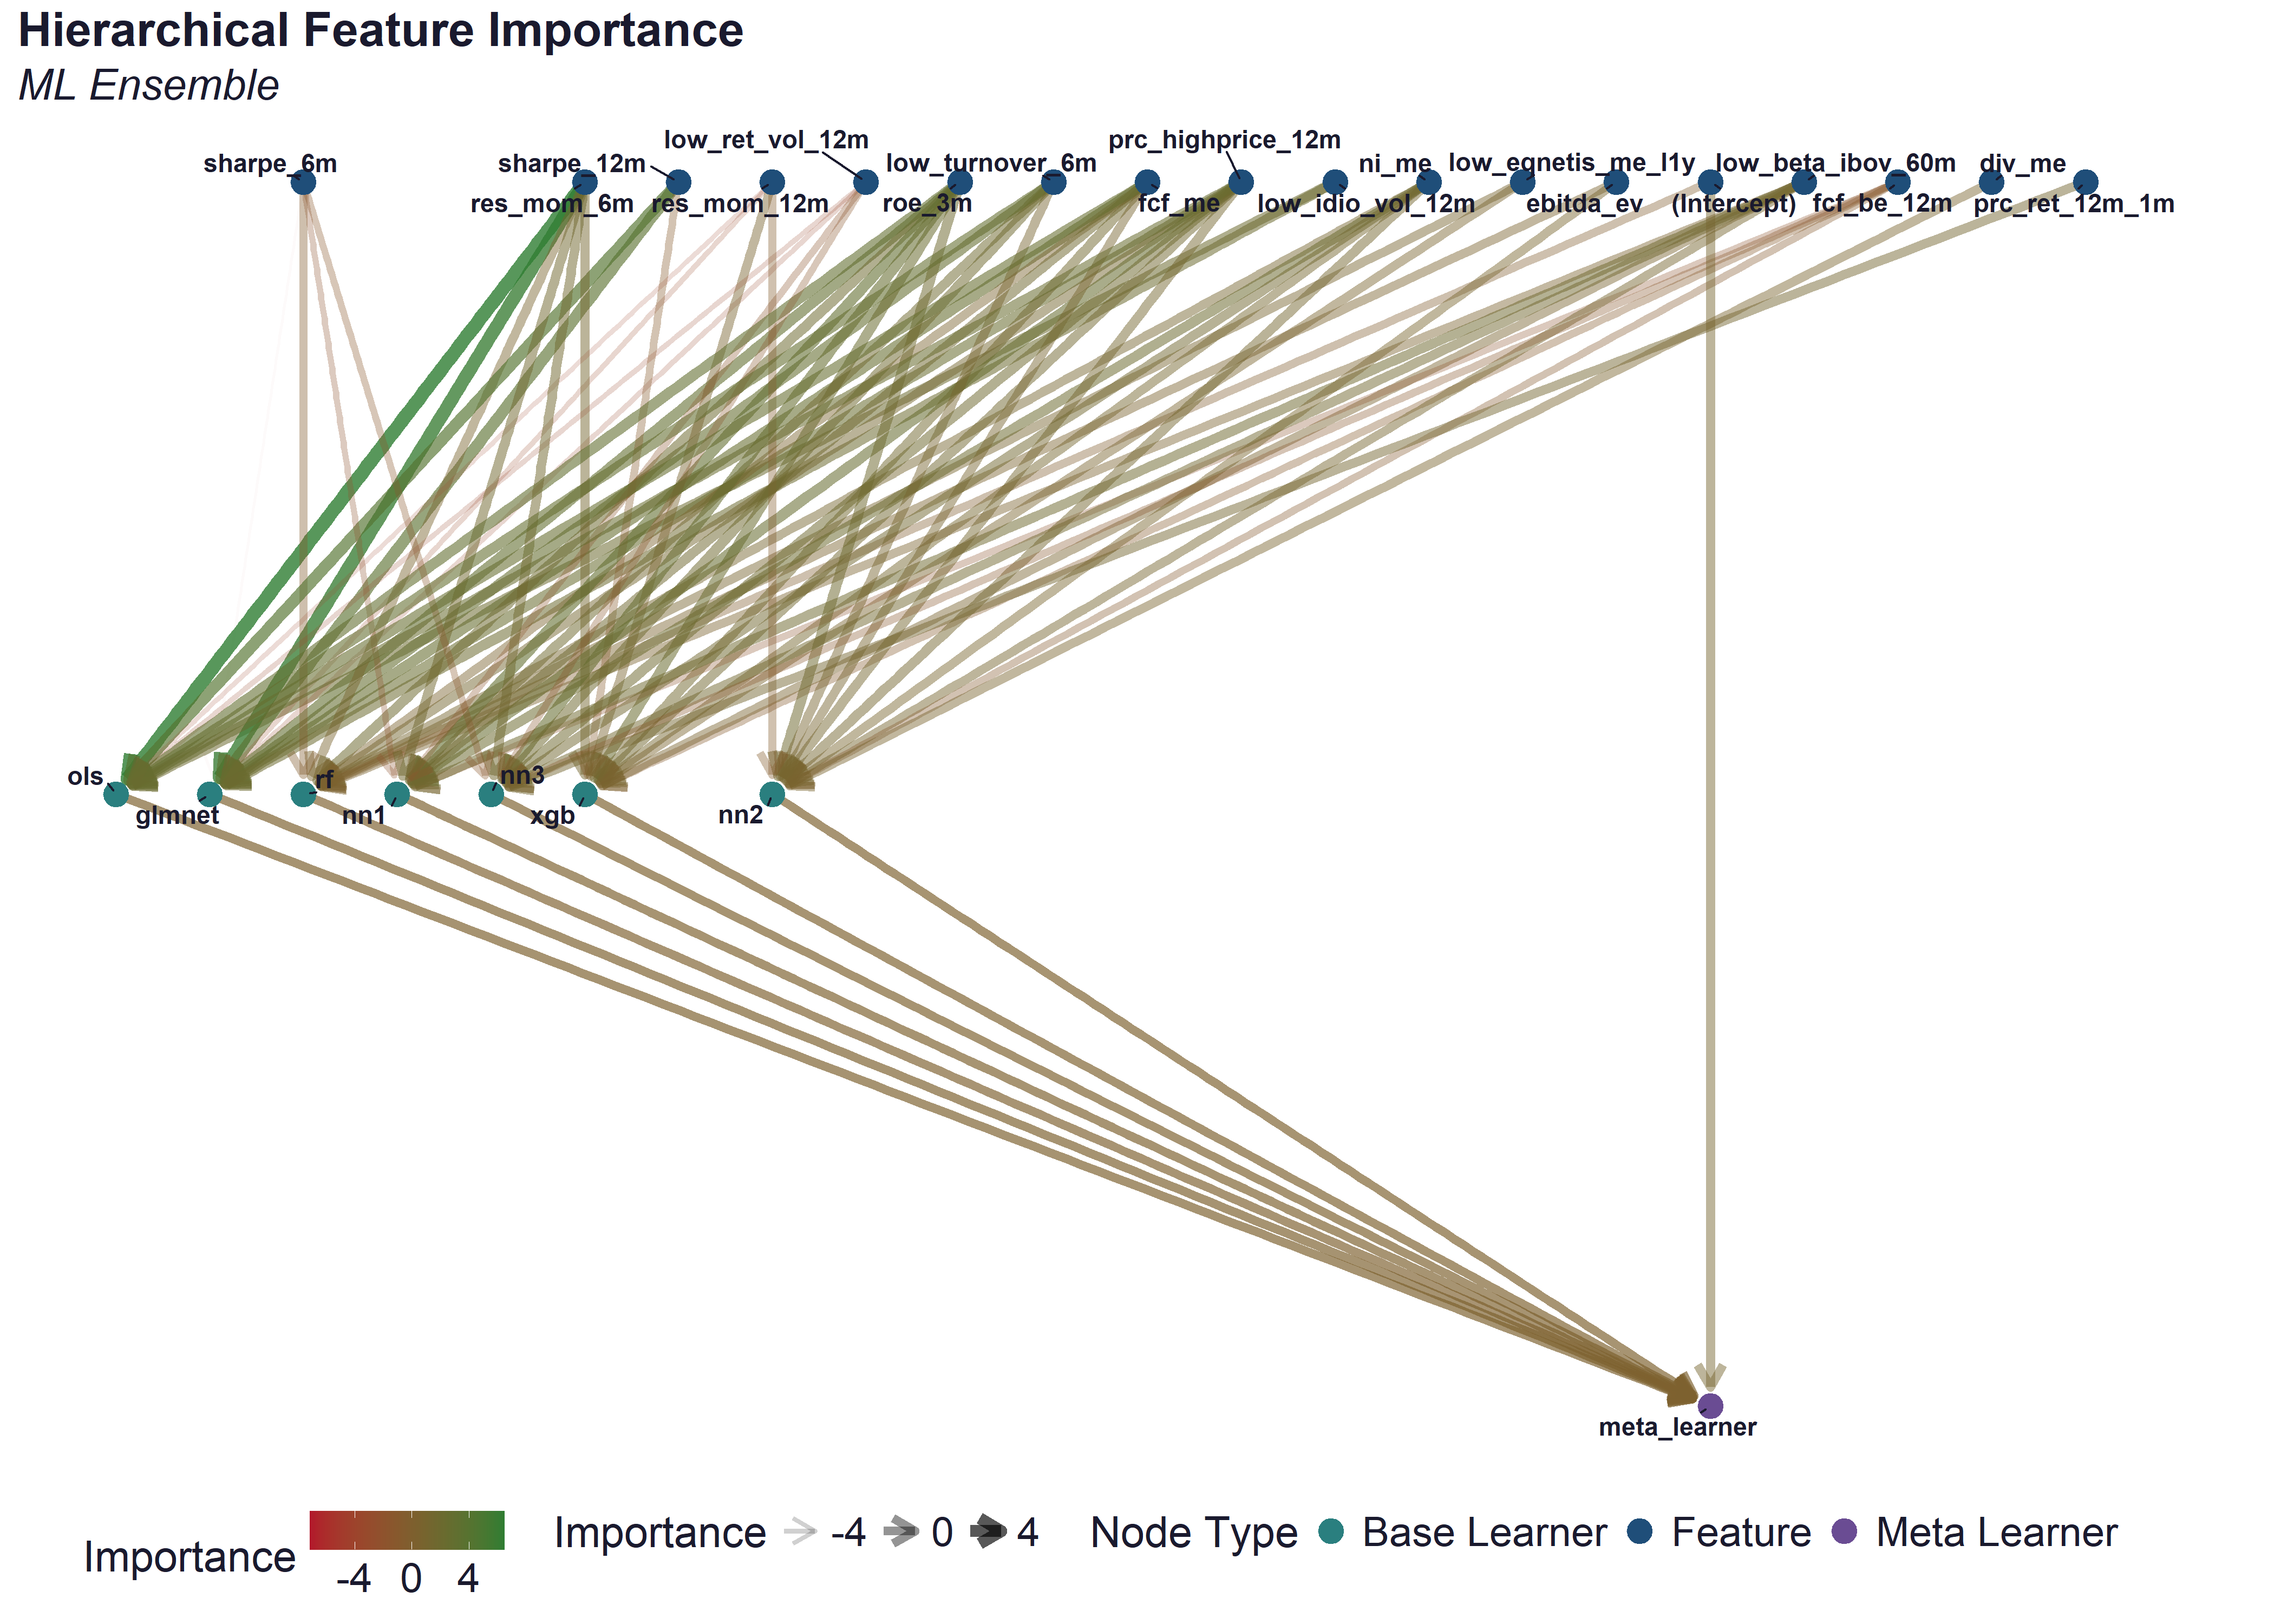
\includegraphics[width=\linewidth]{figures/hierarchical_feature_importance.png}
\label{fig:hier_fi}
\end{figure}
